\documentclass{article} % say
\usepackage{tikz}
\usetikzlibrary{calc,arrows,fit,positioning}


\begin{document}
\tikzset{pop1/.style={blue!40},pop2/.style={red!40}}

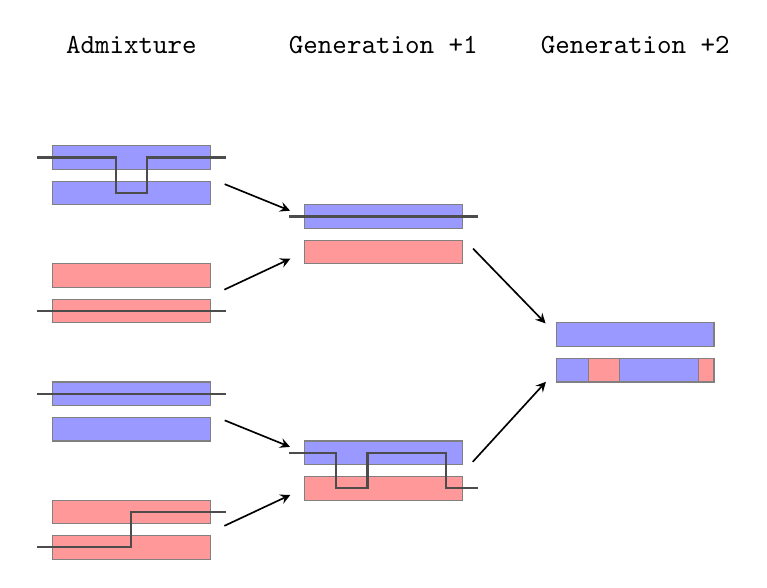
\begin{tikzpicture}[scale=0.2]

\tikzset{
pop1/.style={fill=blue!40,draw=black!50},
pop2/.style={fill=red!40,draw=black!50},
inherit/.style={->,>=stealth,semithick,shorten <=2mm,shorten >=2mm,semithick},
recomb/.style={thick,draw=black!70}
}

% Nodes
\node (hapx) at (1,0) {};
\node (hapy) at (0,1.5) {};
\node (hapxy) at ($10*(hapx) + (hapy)$) {};

\node (gen1) at (0,0) {};
\node (gen2) at ($8*(hapx) + 0*(hapx)$) {};
\node (gen3) at ($8*(hapx) + 8*(hapx)$) {};

\node (ind1gen3) at ($(gen3) + (0,0)$) {};
\node (indsep) at ($5*(hapy)$) {};

\node (ind1gen2) at ($(gen2) + 1*(indsep)$) {};
\node (ind2gen2) at ($(gen2) - 1*(indsep)$) {};

\node (ind1gen1) at ($(gen1) + 1.5*(indsep)$) {};
\node (ind2gen1) at ($(gen1) + 0.5*(indsep)$) {};
\node (ind3gen1) at ($(gen1) - 0.5*(indsep)$) {};
\node (ind4gen1) at ($(gen1) - 1.5*(indsep)$) {};

\node (chr1) at ($0.25*(hapy)$)  {};
\node (chr2) at ($-1.25*(hapy)$) {};


% Haplotypes

\filldraw[pop1] ($(gen1) + (ind1gen1) + (chr1)$) rectangle +(hapxy);
\filldraw[pop1] ($(gen1) + (ind1gen1) + (chr2)$) rectangle +(hapxy);

\filldraw[pop2] ($(gen1) + (ind2gen1) + (chr1)$) rectangle +(hapxy);
\filldraw[pop2] ($(gen1) + (ind2gen1) + (chr2)$) rectangle +(hapxy);

\filldraw[pop1] ($(gen1) + (ind3gen1) + (chr1)$) rectangle +(hapxy);
\filldraw[pop1] ($(gen1) + (ind3gen1) + (chr2)$) rectangle +(hapxy);

\filldraw[pop2] ($(gen1) + (ind4gen1) + (chr1)$) rectangle +(hapxy);
\filldraw[pop2] ($(gen1) + (ind4gen1) + (chr2)$) rectangle +(hapxy);


\filldraw[pop1] ($(gen2) + (ind1gen2) + (chr1)$) rectangle +(hapxy);
\filldraw[pop2] ($(gen2) + (ind1gen2) + (chr2)$) rectangle +(hapxy);

\filldraw[pop1] ($(gen2) + (ind2gen2) + (chr1)$) rectangle +(hapxy);
\filldraw[pop2] ($(gen2) + (ind2gen2) + (chr2)$) rectangle +(hapxy);


\filldraw[pop1] ($(gen3) + (ind1gen3) + (chr1)$) rectangle +(hapxy);
\fill[pop1] ($(gen3) + (ind1gen3) + (chr2)$) rectangle +(hapxy);
\fill[pop2] ($(gen3) + (ind1gen3) + (chr2)+ 2*(hapx)$) rectangle ($(gen3) + (ind1gen3) + (chr2)+ (hapxy)$);
\fill[pop1] ($(gen3) + (ind1gen3) + (chr2)+ 4*(hapx)$) rectangle ($(gen3) + (ind1gen3) + (chr2)+ (hapxy)$);
\fill[pop2] ($(gen3) + (ind1gen3) + (chr2)+ 9*(hapx)$) rectangle ($(gen3) + (ind1gen3) + (chr2)+ (hapxy)$);
%\draw ($(gen3) + (ind1gen3) + (chr2)$) rectangle +(hapxy);


% Copying lines

\node (startline) at ($-1*(hapx) + 0.5*(hapy)$) {};
\node (chrdiff) at ($(chr1) - (chr2)$) {};

\node (hapx) at (1,0) {};

\draw[recomb] ($(gen1) + (ind1gen1) + (chr1) + (startline)$) -- ++($(hapx)$) --  ++($4*(hapx)$) --  ++($-1*(chrdiff)$) -- ++($2*(hapx)$) -- ++($(chrdiff)$) -- ++($4*(hapx)$) -- ++($1*(hapx)$);
\draw[recomb] ($(gen1) + (ind2gen1) + (chr2) + (startline)$) -- ++($(hapx)$) -- ++($10*(hapx)$) --  ++($(hapx)$);
\draw[recomb] ($(gen1) + (ind3gen1) + (chr1) + (startline)$) -- ++($(hapx)$) -- ++($10*(hapx)$) --  ++($(hapx)$);
\draw[recomb] ($(gen1) + (ind4gen1) + (chr2) + (startline)$) -- ++($(hapx)$) --  ++($5*(hapx)$) --  ++($(chrdiff)$) -- ++($2*(hapx)$) -- ++($3*(hapx)$) -- ++($1*(hapx)$);

\draw[recomb] ($(gen2) + (ind1gen2) + (chr1) + (startline)$) -- ++($(hapx)$) -- ++($10*(hapx)$) --  ++($(hapx)$);
\draw[recomb] ($(gen2) + (ind2gen2) + (chr1) + (startline)$) -- ++($(hapx)$) --  ++($2*(hapx)$) --  ++($-1*(chrdiff)$) -- ++($2*(hapx)$) -- ++($(chrdiff)$) -- ++($3*(hapx)$) -- ++($2*(hapx)$) -- ++($-1*(chrdiff)$) -- ++($(hapx)$) -- ++($(hapx)$) ;


% Arrows
\draw[inherit] ($(gen1) + (ind1gen1) + (chr2) + 10*(hapx) + 0.75*(chrdiff)$) -- ($(gen2) + (ind1gen2) + (chr1) + 0.5*(hapy)$);
\draw[inherit] ($(gen1) + (ind2gen1) + (chr2) + 10*(hapx) + 0.75*(chrdiff)$) -- ($(gen2) + (ind1gen2) + (chr2) + 0.5*(hapy)$);
\draw[inherit] ($(gen1) + (ind3gen1) + (chr2) + 10*(hapx) + 0.75*(chrdiff)$) -- ($(gen2) + (ind2gen2) + (chr1) + 0.5*(hapy)$);
\draw[inherit] ($(gen1) + (ind4gen1) + (chr2) + 10*(hapx) + 0.75*(chrdiff)$) -- ($(gen2) + (ind2gen2) + (chr2) + 0.5*(hapy)$);

\draw[inherit] ($(gen2) + (ind1gen2) + (chr2) + 10*(hapx) + 0.75*(chrdiff)$) -- ($(gen3) + (ind1gen3) + (chr1) + 0.5*(hapy)$);
\draw[inherit] ($(gen2) + (ind2gen2) + (chr2) + 10*(hapx) + 0.75*(chrdiff)$) -- ($(gen3) + (ind1gen3) + (chr2) + 0.5*(hapy)$);


% Labels
\node (lab1) at ($(gen1) + 2.5*(indsep) + 0.5*(hapxy)$) {$\texttt{Admixture}$};
%\node (lab2) at ($(gen2) + 2.5*(indsep) + 0.5*(hapxy)$) {$\texttt{Generation 1}$};
\node (lab2) at ($2*(gen2) + 2.5*(indsep) + 0.5*(hapxy)$) {$\texttt{Generation +1}$};
\node (lab3) at ($4*(gen2) + 2.5*(indsep) + 0.5*(hapxy)$) {$\texttt{Generation +2}$};

\end{tikzpicture}
\end{document}